\documentclass[a4paper]{article}
\usepackage[letterpaper, margin=1in]{geometry} % page format
\usepackage{listings} % this package is for including code
\usepackage{graphicx} % this package is for including figures
\usepackage{amsmath}  % this package is for math and matrices
\usepackage{amsfonts} % this package is for math fonts
\usepackage{tikz} % for drawings
\usepackage{hyperref} % for urls
\usepackage{stackengine}
\usepackage[autostyle]{csquotes}

\newcommand\tab[1][0.5cm]{\hspace*{#1}}

\title{Midterm Exam}
\author{Kaitlyn Mulligan}
\date{3/13/19}

\begin{document}
\lstset{language=Python}

\maketitle

\section{Instructions}
This test could be written in \LaTeX, just as all the homework assignments.  Write in 
understandable, easy to follow English.  Make sure you provide good illustrations and 
figures.  Remember to include your Python programs in your assignment.\\
\tab Your assignment should be submitted in two ways: through GitHub, and in hardcopy (in 
class).  Use the \textbf{same} repository you have been using and submit your work in a 
folder named "\verb|lastname-midterm|", where lastname is your last name.

% ----------------------------------------------------------------------------------------------

\section{Problem Set}
The following is a list of problems you will work on.  When providing your solutions (hopefully 
using \LaTeX), do not simply give the final answer, show how you arrived to the solution, justify 
your assumptions, and explain your results clearly.

% ----------------------------------------------------------------------------------------------

\subsection{1} Compare two algorithms on a classification task: the Pocket algorithm (designed 
for classification), and linear regression (not designed for classification).  For linear 
regression, after learning the weights \textbf{w}; we use \textit{h}(\textbf{x}) = sign
(\textbf{w}$^T$\textbf{x}) to classify \textbf{x}.  For the dataset, start by using the following 
Python code:
\lstinputlisting[language=Python,frame=single]{midterm.generate.py}
Create another dataset using the same method as above but now you will classify between 4 and the 
rest of the numbers.  To do this you should change lines 8 and 9 as follows:\\
\verb|y[y<>4] = -1|\\
\verb|y[y==4] = +1|\\
Try the following three approaches using the dataset with the new changes, plot the final (best) 
hypothesis on each and then explain which works best in terms both $E_{\text{out}}$ and the 
amount of computation required.  E.g., what is the final classification error?  after how many 
iterations did you stop the Pocket algorithm?\\

First I created another data set using the same method as above and utilized it in my Perceptron 
Learning Algorithm.  The code I used for the next three parts can be seen below.  You can find the 
data given in the question in the data section of the main method.  For each part, the only changes 
that were made were to comment/uncomment specific lines of the code which I will metion below.
\lstinputlisting[language=Python,frame=single]{midterm-1.py}
\begin{itemize}
    \item[(a)] The Pocket algorithm, starting from \textbf{w}=0.\\
    To implement the Pocket algorithm, starting from \textbf{w}=0, I commented out the lines in the 
    linear regression section, initialized the weights to zero with the line \verb|w = np.zeros(3)|, and 
    commented out the line \verb|w=wlr|.  I stopped the Pocket Algorithm after 10,000 iterations.  Below 
    is a plot of the final hypothesis.  The final classification error was 1063.
    \begin{center}
        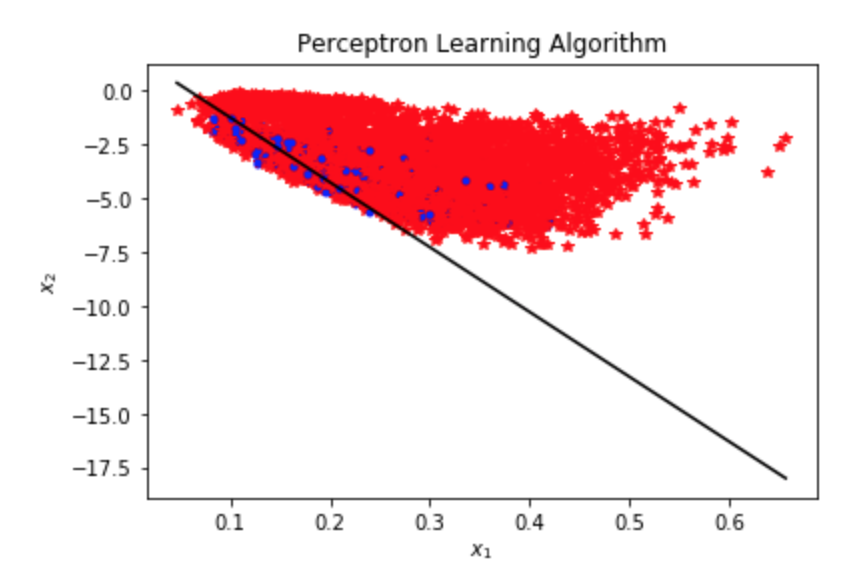
\includegraphics[width=0.6\textwidth]{a-Pocket.jpg}
    \end{center}
    \item[(b)] Linear regression (applied as a classification method).\\
    To implement Linear Regression, I uncommented the lines in the linear regression section.  
    After the return statement the algorithm will stop running so I do not need to comment or 
    uncomment any lines in that section.  Below is a plot of the final hypothesis.
    \begin{center}
        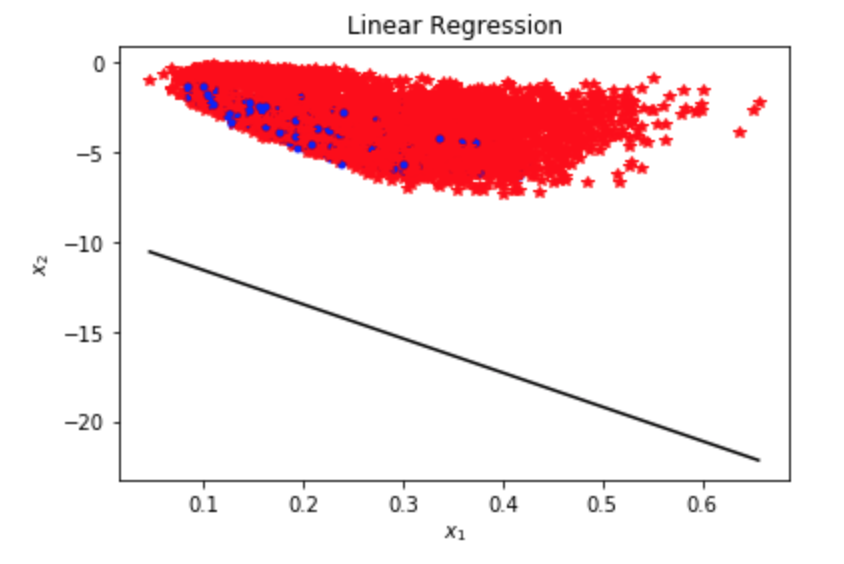
\includegraphics[width=0.6\textwidth]{b-LinReg.jpg}
    \end{center}
    \item[(c)] The Pocket algorithm, starting from the solution given by linear regression.\\
    To implement the Pocket algorithm, starting from the solution given by linear regression, I 
    uncommented the first two lines of the linear regression section and commented the two lines: 
    \verb|pltPer(X,y,wlr)| and \verb|return|.  I then commented the line \verb|w=np.zeros(3)| 
    and uncommented the line \verb|w=wlr|.  I stopped the Pocket Algorithm after 10,000 iterations.  
    Below is a plot of the final hypothesis.  The final classification error was 652.
    \begin{center}
        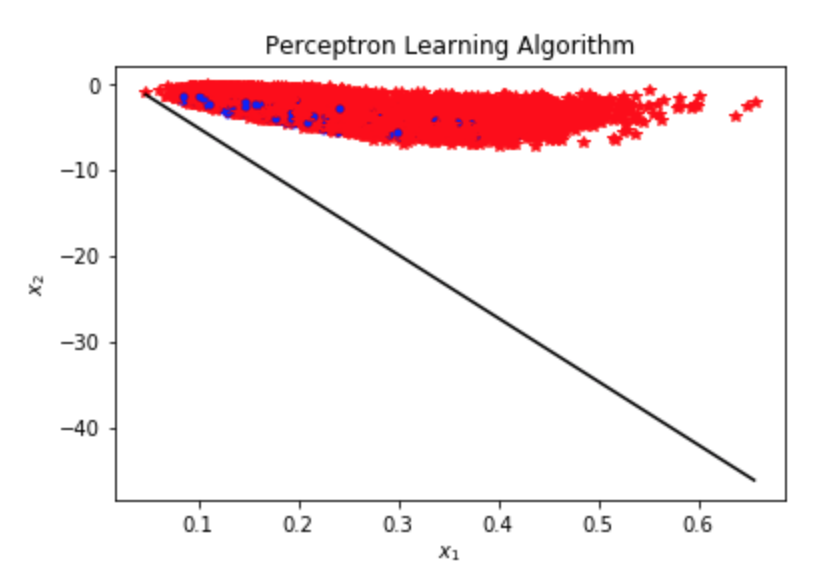
\includegraphics[width=0.6\textwidth]{c-Pocket.jpg}
    \end{center}
\end{itemize}

% ----------------------------------------------------------------------------------------------

\subsection{2} Write a Python program that solves \textbf{Problem 2.12} in an iterative manner.  
If you are feeling adventurous, plot the values of $N$ as the program converges to a steady 
value of N.\\

Problem 2.12 states:
\begin{displayquote}
For an $\mathcal{H}$ with $d_{VC} = 10$, what sample size do you 
need (as prescribed by the generalization bound) to have $95\%$ confidence that your 
generalization error is at most $0.05$?
\end{displayquote}
Having already answered this question in a previous homework assignment, we know that the value 
of $N$ should be converging to approximately $452956$.  To solve this in an iterative manner, 
we can use the following Python program which utilizes Equation (2.13) and the given values.
\lstinputlisting[language=Python,frame=single]{midterm-2.py}
After 20 iterations, this Python program returns a value of $N = 452956.8647230992$.  Feeling 
adventurous, I decided to plot the values of $N$ as the program converges to a steady value of 
$N$.  I decided to write the code for the plot in the code above.  The resulting plot of $N$ 
is below.
\begin{center}
    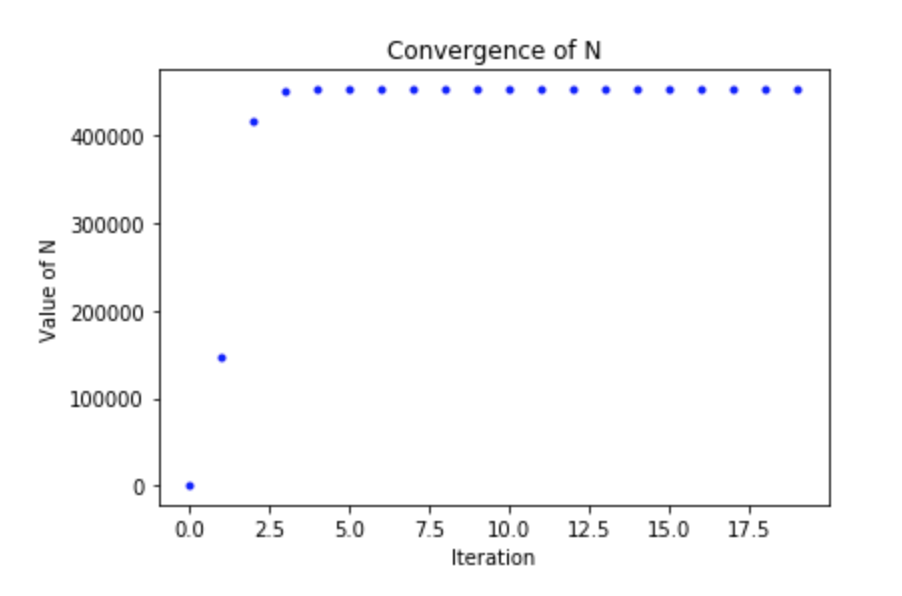
\includegraphics[width=0.6\textwidth]{NConvergence.jpg}
\end{center}

% ----------------------------------------------------------------------------------------------

\subsection{3 (extra credit)} Albert Einstein said "Creativity is intelligence having fun".  You 
are very smart and talented.  That is why you are in this class.  With that in mind... I recently 
acquired the domain name  "\verb|marist.ai|" and I am looking to create site for students and 
faculty to share their AI-related projects; so, for a chance to be displayed our future website, 
draw some type of logo for the new site here:
\begin{center}
    \fbox{\begin{minipage}{2.5in}\hfill\vspace{2.5in}\end{minipage}}
\end{center}

\end{document}
